\documentclass[9pt,table]{beamer}

\usepackage[slovene]{babel}
\usepackage[utf8]{inputenc}
\usepackage[T1]{fontenc}
\usepackage{lmodern}
\usepackage{graphicx}

\usetheme{Berlin}
\usecolortheme{beaver}
\useoutertheme{infolines}


\begin{document}

% ===================================================================

\title{Samodejno odvajanje}
\author{Andrej Borštnik, Barbara Bajcer}
\institute[FMF]{Fakulteta za matematiko in fiziko}

\begin{frame}
   \titlepage
\end{frame}

% -------------------------------------------------------------------

\begin{frame}
   \frametitle{Kratek pregled}
   \tableofcontents[pausesections]
\end{frame}

% ===================================================================

\section{Samodejno odvajanje}

\begin{frame}
\frametitle{}
\begin{center}
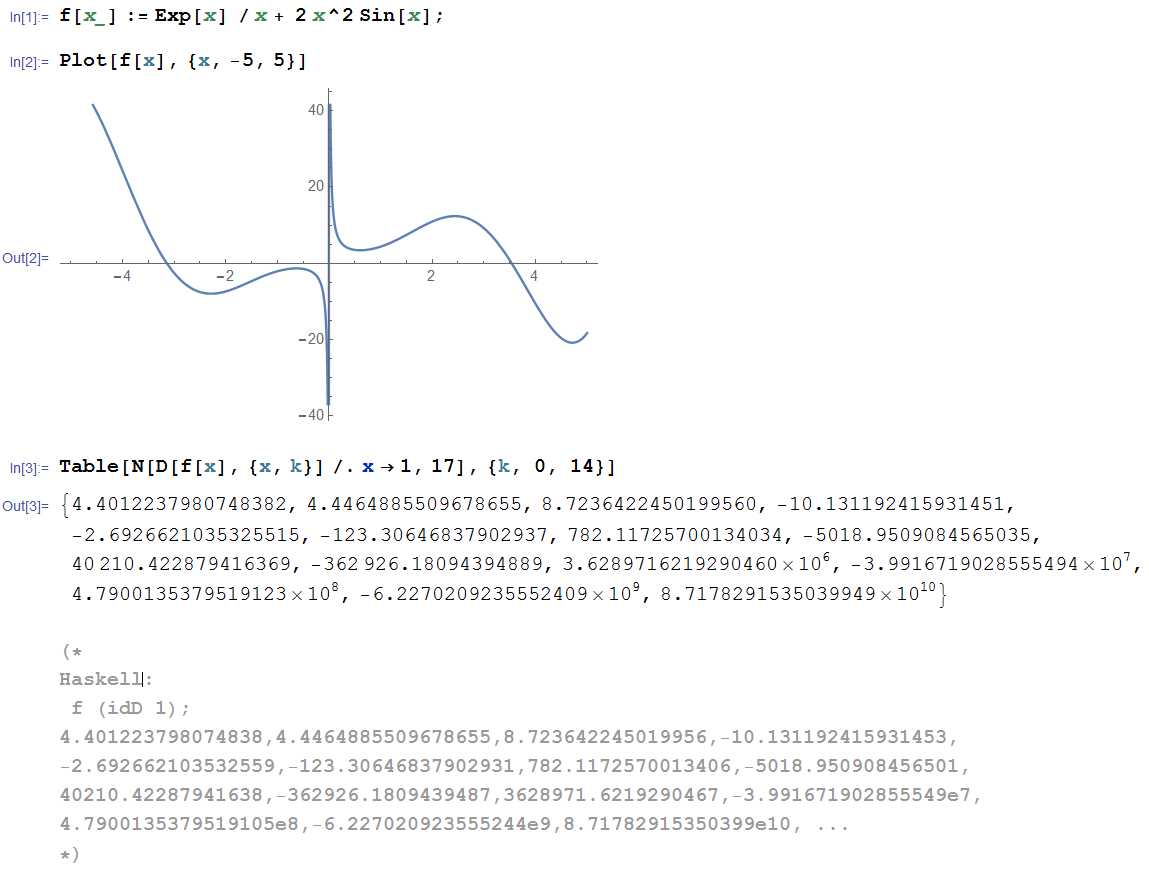
\includegraphics[width=11.5cm]{graf1.png}
\end{center}
\end{frame}

\begin{frame}
\frametitle{}
\begin{center}
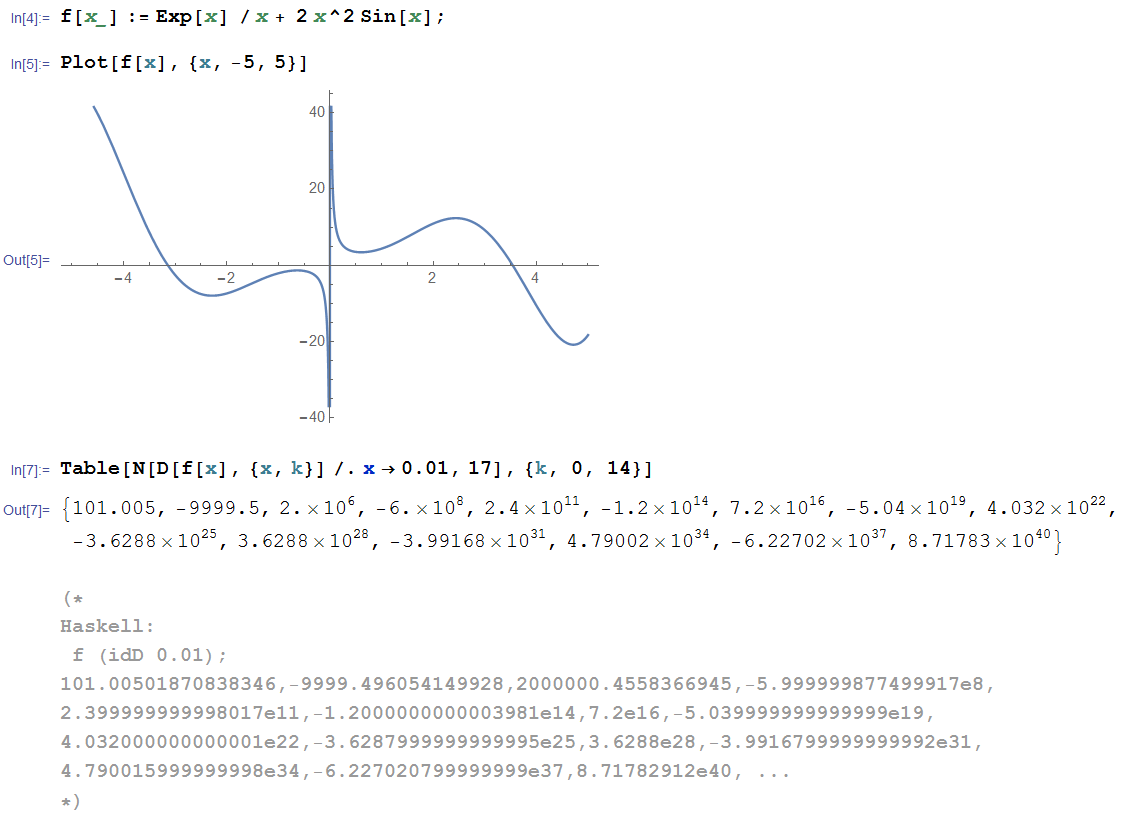
\includegraphics[width=12cm]{graf2.png}
\end{center}
\end{frame}

\begin{frame}[fragile]
\frametitle{}
\pause
\begin{verbatim}
g(x) = x^2
g (idD 4)
16.0, 8.0, 2.0, 0
\end{verbatim}\pause
\begin{verbatim}
h(x) = x^6
h (idD 1)
1.0, 6.0, 30.0, 120.0, 360.0, 720.0, 720.0, 0
\end{verbatim}\pause
\begin{verbatim}
k(x) = sin(x^2)
k (idD 1)
0.8414709848078965, 1.0806046117362795, -2.2852793274953065, 
-14.420070264639875, -22.568626742439122, 87.08875465286715, 
746.5137961465103, 2028.9913034612805, -4355.06268259366, 
-69627.83387598622, -308672.6345339131, Interrupted.
\end{verbatim}\pause
Kjer funkcija ni odvedljiva, dobimo čudne stvari:\pause
\begin{verbatim}
f (idD 0)
Infinity, NaN, NaN, NaN, NaN, NaN, NaN, NaN, NaN, NaN, NaN, NaN, NaN, 
NaN, NaN, NaN, NaN, ...
\end{verbatim}
\end{frame}

% -------------------------------------------------------------------

\section{Levi in desni odvodi}

\begin{frame}[fragile]
\frametitle{}
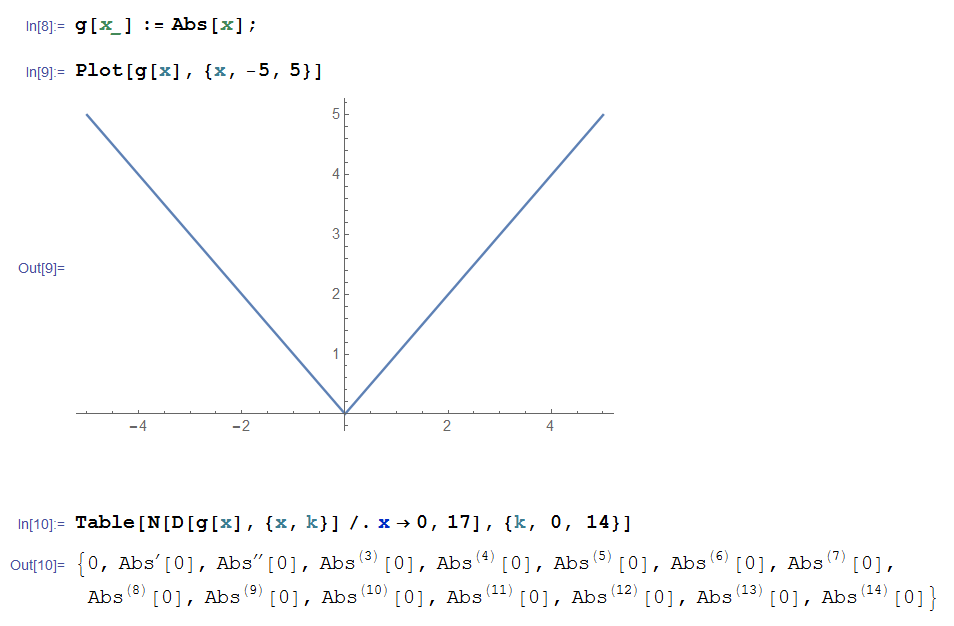
\includegraphics[width=10cm]{graf3.png}

\pause
Haskell:
\begin{verbatim}
g (idD 0)
D 0.0 -1.0 1.0
\end{verbatim}
\end{frame}

\begin{frame}[fragile]
\frametitle{}
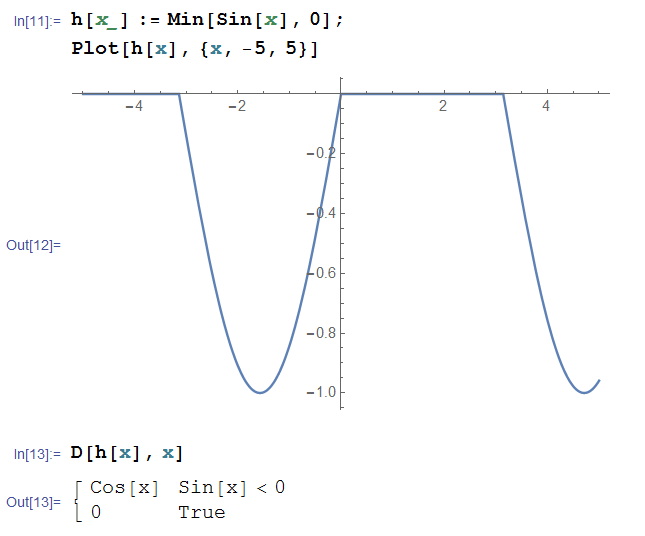
\includegraphics[width=8cm]{graf4.png}

\pause
Haskell:
\begin{verbatim}
h (idD 0)
D 0.0 1.0 0.0
\end{verbatim}
\end{frame}

% -------------------------------------------------------------------

\section{Lipschitzove konstante}

\begin{frame}
\frametitle{}

\end{frame}



\end{document}